\documentclass{beamer}
\usepackage[ngerman]{babel}
\usepackage[utf8x]{inputenc}
\usepackage{amsmath, amsfonts, amssymb}
\usepackage{tikz}
\usepackage{pgfplots}
\usepackage{xcolor}
\usepackage{subcaption}

\usetheme{Luebeck}
\useinnertheme{rounded}
\usefonttheme{professionalfonts}
\setbeamercovered{transparent}
\beamertemplatenavigationsymbolsempty
\setbeamertemplate{footline}{%
  \begin{beamercolorbox}[wd = 0.5\textwidth, ht = 3ex, dp = 1.5ex, leftskip = .5em, rig htskip = .5em]{author in head/foot}%
    \usebeamerfont{author in head/foot}%
    \insertframenumber/\inserttotalframenumber\hfill\insertshortauthor%
  \end{beamercolorbox}%
  \vspace*{-4.5ex}\hspace*{0.5\textwidth}%
  \begin{beamercolorbox}[wd = 0.5\textwidth, ht = 3ex, dp = 1.5ex, left, leftskip = .5em]{title in head/foot}%
    \usebeamerfont{title in head/foot}%
    \insertshorttitle%
\end{beamercolorbox}}

\renewcommand{\arraystretch}{1.3}

\title{Multi-Gigabit Complex Sub-Nyquist Sampling SDR for 60 GHz}
\subtitle{Master Thesis at the Telecommunications Circuits Lab, EPFL}
\author{Lorenz Koestler $ < $lorenzk@ee.ethz.ch$ > $}
\date[1.9..2013]{1. September 2014}

\newcommand{\mc}[2]{\multicolumn{#1}{c|}{#2}}

\begin{document}

\begin{frame}
  \titlepage

  Advisors: \\
  Nicholas Preyss $ < $\href{mailto:nicholas.preyss@epfl.ch}{nicholas.preyss@epfl.ch}$ > $ \\
\end{frame}

\begin{frame}{Introduction}
  \begin{itemize}
  \item Mobile communication systems became ubiquitous
  \item Essential importance that network throughput increases
    logarithmically
  \item Higher spectral efficiency (channel allocation, MIMO etc.) is possible
  \item Use new frequency bands
  \item 60 GHz ISM band, which defines 1.76 GHz wide channels
  \item Possibility for big antenna arrays on small surface
  \item High free space path loss allows reusage of channel
  \item New Applications: lossless, uncompressed HD video streams,
    high density cell networks (5G)
  \end{itemize}
\end{frame}

\begin{frame}{Goal}
  \begin{itemize}
  \item Analyze different receiver designs
  \item Implement a versatile simulation and test setup to analyze designs
  \item Measure channel characteristics like delay spread, phase noise etc.
  \item Make a demo setup to show that high data rates using high QAM modulation
    are possible
  \item Find performance limiting impairments for 60 GHz communication systems
  \end{itemize}
\end{frame}

\begin{frame}{Receiver Designs}
  \begin{columns}[T]
    \begin{column}{.5\textwidth}
      \begin{block}{Goal}
        \begin{itemize}
        \item Digitize the channel of interest with as high as possible
          dynamic range
        \item Suppress influence of other channels
        \end{itemize}
      \end{block}
    \end{column}
    \begin{column}{.5\textwidth}
      \begin{block}{Challenge}
        \begin{itemize}
        \item Channel width is as high as the available ADC sampling
          speeds -> Oversampling is not easily possible
        \item
          Channel width can be bigger of IF frequency
          (1.8 GHz wide channel on IF center frequency of 1 GHz)
        \item Many component restrictions exist
        \end{itemize}
      \end{block}
    \end{column}
  \end{columns}
\end{frame}

\begin{frame}{Direction Conversion / High IF Receiver}
  \only<1>{
    \begin{columns}[T]
      \begin{column}{.6\textwidth}
        \includegraphics[width=\textwidth]{figures/rx_4_bd}
      \end{column}
      \begin{column}{.4\textwidth}
        \begin{block}{Direction Conversion}
          \begin{itemize}
          \item Most popular RX Architecture for SDRs
          \item 60 GHz RF frontend does not go below 1 GHz
          \end{itemize}
        \end{block}
      \end{column}
    \end{columns}
    \vspace{4ex}
  }
  \only<2>{
    \begin{columns}[T]
      \begin{column}{.5\textwidth}
        \includegraphics[width=\textwidth]{figures/rx_rf_0_freq_s}
      \end{column}
      \begin{column}{.5\textwidth}
        \includegraphics[width=\textwidth]{figures/rx_rf_0_freq_i}
      \end{column}
    \end{columns}
    \vspace{11ex}
  }
  \begin{columns}[T]
    \begin{column}{.6\textwidth}
      \includegraphics[width=\textwidth]{figures/rx_0_bd}
    \end{column}
    \begin{column}{.4\textwidth}
      \begin{block}{High IF Receiver}
        \begin{itemize}
        \item Second mixer must run at 5 GHz
        \item DC-Block blocks part of signal
        \end{itemize}
      \end{block}
    \end{column}
  \end{columns}
\end{frame}


\begin{frame}{Quadrature Intermediate Frequency Sub-Nyquist Sampling Receiver}
  \includegraphics[width=\textwidth]{figures/rx_3_bd} \\

  \begin{block}{xxx}
    \begin{itemize}
    \item Uses only one mixer stage
    \item Higher analog than digital bandwidht of ADC allows for Sub-Nyquist Sampling
    \item Channel-dependent, Frequency selectivity leads to non linear error
    \end{itemize}
  \end{block}
\end{frame}

\begin{frame}{$90^\circ$ Coupler / Hilbert Transform}
  \begin{columns}[T]
    \begin{column}{.5\textwidth}
      \begin{block}{Time Domain}
        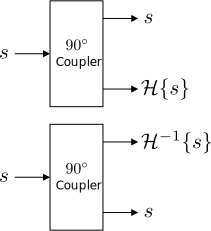
\includegraphics[width=\textwidth]{figures/90deg_coupler_hilbert}
      \end{block}
    \end{column}
    \begin{column}{.5\textwidth}
      \begin{block}{Frequency Domain}
        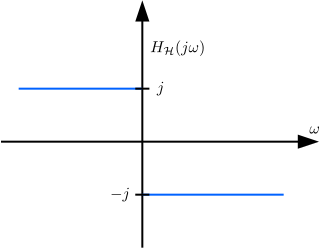
\includegraphics[width=\textwidth]{figures/hilbert}
      \end{block}
    \end{column}
  \end{columns}
\end{frame}

\begin{frame}{Image Rejection using $90^\circ$ Couplers}
  \begin{columns}[T]
    \begin{column}{.5\textwidth}
      \only<1-2>{
        \includegraphics[width=\textwidth]{figures/rx_rf_1_freq_s}
        \vspace{-5mm}
        \[r(t)\]
      }

      \only<2-3>{
        \vspace{5mm}
        \includegraphics[width=\textwidth]{figures/rx_rf_1_freq_a}
        \vspace{-5mm}
        \[a(t) = \text{LP}\{r(t) \cdot \cos(2\pi \cdot f_{\text{RX LO}} \cdot t)\}\]
      }

      \only<3>{
        \vspace{5mm}
        \includegraphics[width=\textwidth]{figures/rx_rf_1_freq_Hb}
        \vspace{-5mm}
        \[\mathcal{H}^{-1}\{b\}(t)\]
      }
    \end{column}
    \begin{column}{.5\textwidth}
      \only<1-2>{
        \includegraphics[width=\textwidth]{figures/rx_rf_1_freq_Hs}
        \vspace{-5mm}
        \[\mathcal{H}^{-1}\{r\}(t)\]
      }

      \only<2-3>{
        \vspace{5mm}
        \includegraphics[width=\textwidth]{figures/rx_rf_1_freq_b}
        \vspace{-5mm}
        \[b(t) = \text{LP}\{r(t) \cdot \sin(2\pi \cdot f_{\text{RX LO}} \cdot t)\}\]
      }

      \only<3>{
        \vspace{5mm}
        \includegraphics[width=\textwidth]{figures/rx_rf_1_freq_c}
        \vspace{-5mm}
        \[c(t) = a(t) + \mathcal{H}^{-1}\{b\}(t)\]
      }
    \end{column}
  \end{columns}

  \only<1>{
    \vspace{1.5cm}
    \includegraphics[width=\textwidth]{figures/rx_rf_1_bd}
  }
\end{frame}

\begin{frame}{Quadrature Intermediate Frequency Sub-Nyquist Sampling}
  \begin{columns}[T]
    \begin{column}{.5\textwidth}
      \only<1-2>{
        \includegraphics[width=\textwidth]{figures/rx_adc_3_c}
        \vspace{-5mm}
        \[c(t)\]
      }

      \only<2-3>{
        \vspace{5mm}
        \includegraphics[width=\textwidth]{figures/rx_adc_3_d0}
        \vspace{-5mm}
        \[d_0[k] = c(k/f_s) \]
      }

      \only<3-4>{
        \vspace{5mm}
        \includegraphics[width=\textwidth]{figures/rx_adc_3_jd0}
        \vspace{-5mm}
        \[j \cdot d_0[k]\]
      }
    \end{column}
    \begin{column}{.5\textwidth}
      \only<1-2>{
        \includegraphics[width=\textwidth]{figures/rx_adc_3_Hc}
        \vspace{-5mm}
        \[\mathcal{H}^{-1}\{c\}(t)\]
      }

      \only<2-3>{
        \vspace{5mm}
        \includegraphics[width=\textwidth]{figures/rx_adc_3_d1}
        \vspace{-5mm}
        \[d_1[k] = \mathcal{H}^{-1}\{c\}(k/f_s)\]
      }

      \only<3-4>{
        \vspace{5mm}
        \includegraphics[width=\textwidth]{figures/rx_adc_3_e}
        \vspace{-5mm}
        \[e[k] = d_1[k] + j \cdot d_0[k] \]
      }
    \end{column}
  \end{columns}
  \only<1>{
    \vspace{1.5cm}
    \centering
    \includegraphics[width=0.6\textwidth]{figures/rx_adc_3_bd}
  }

  \only<4>{
    \centering
    \includegraphics[width=0.5\textwidth]{figures/rx_adc_3_f}
    \[-j \cdot e[k]\]
  }
\end{frame}

\begin{frame}{FPGA - Design}
  \begin{columns}[T]
    \begin{column}{.5\textwidth}
      \begin{block}{Tasks}
        \begin{itemize}
        \item Acquire Data from ADC
        \item Store Data in real-time
        \item Provide download to PC
        \end{itemize}
      \end{block}
      TODO: add pic of FPGA board
    \end{column}
    \begin{column}{.5\textwidth}
      \begin{block}{Data Storage Speed}
        \begin{itemize}
        \item ADC delivers one 12-bit channel at 3.6 GHz or
          two 12-bit channels at 1.8 GHz $\rightarrow 5.4 \;\text{GB}/\text{s}$.
        \item DDR3 Ram 64 bits at 500 MHz DDR $\rightarrow 8 \;\text{GB}/\text{s}$.
          (P\&R difficult at 800 MHz)
        \end{itemize}
      \end{block}
      \begin{block}{Download Speed}
        \begin{itemize}
        \item USB-to-UART bridge is limited to $1 \text{Mbit}/\text{s}$
        \item Download of 1 GiB takes approx. 18 minutes
        \item USB 2.0 can to up to $480 \;\text{Mbit}/\text{s}$, reached speed
          about $140 \;\text{Mbit}/\text{s}$ $\rightarrow$ download in about 1 minute
        \end{itemize}
      \end{block}
    \end{column}
  \end{columns}
\end{frame}

\begin{frame}{FPGA - Architecture}
  \only<1>{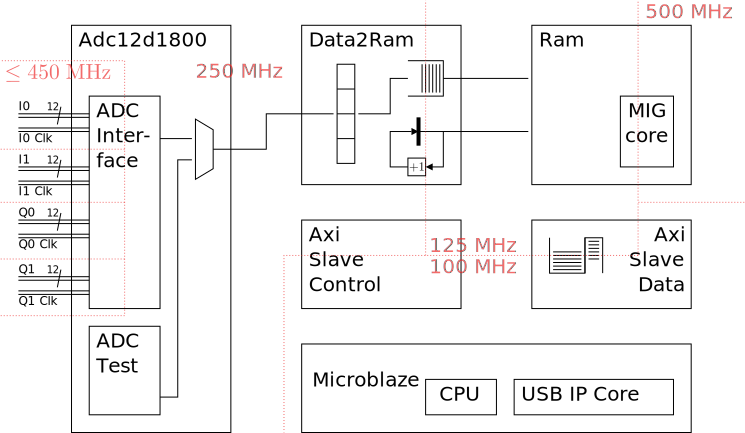
\includegraphics[width=\textwidth]{figures/fpga_architecture_overview}}
  \only<2>{\includegraphics[width=\textwidth]{figures/fpga_clock_domains_overview}}
\end{frame}

\begin{frame}{FPGA - ADC Interface}
  \begin{columns}[T]
    \begin{column}{.7\textwidth}
      \begin{figure}
        \centering
        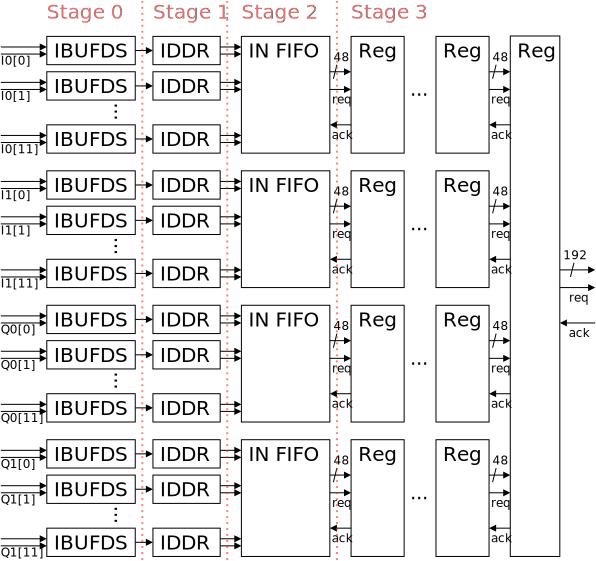
\includegraphics[width=\textwidth]{figures/fpga_adc}
      \end{figure}
    \end{column}
    \begin{column}{.3\textwidth}
      \begin{block}{Stage 0}
        LVDS to single ended
      \end{block}
      \begin{block}{Stage 1}
        Double to Single Data Rate
      \end{block}
      \begin{block}{Stage 2}
        Clock boundary 450 MHz to 250 MHz
      \end{block}
      \begin{block}{Stage 3}
        Centralization and Reordering
      \end{block}
    \end{column}
  \end{columns}
\end{frame}

\begin{frame}{FPGA - Reset Distribution}
  \begin{columns}[T]
    \begin{column}{.4\textwidth}
      \begin{block}{Challenge}
        Release asynchronous reset accross multiple
        clock domains in same cylce on whole FPGA die
      \end{block}

      \begin{block}{Solution}
        \begin{itemize}
        \item Reset Synchronizers
        \item Global 5 MHz reset distribution clock
        \item Two global reset trees
        \end{itemize}
      \end{block}
    \end{column}
    \begin{column}{.6\textwidth}
      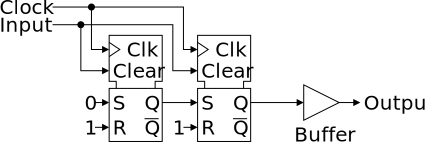
\includegraphics[width=\textwidth]{figures/RstSync} \\
      \vspace{4ex}
      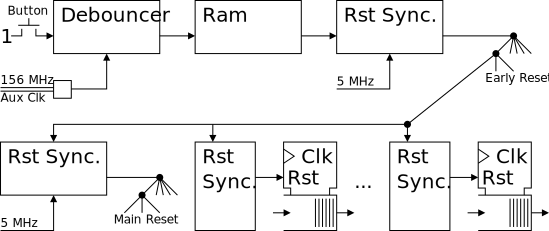
\includegraphics[width=\textwidth]{figures/rst_generation}
    \end{column}
  \end{columns}
\end{frame}

\begin{frame}{Test-Setup Block Diagram}
  \includegraphics[width=\textwidth]{figures/res_450_setup}
\end{frame}

\begin{frame}{Test-Setup Picture}
  \includegraphics[width=\textwidth]{pictures/res_450_setup}
\end{frame}

\begin{frame}{Phase Noise, First Results at 450 MS / s}
  \begin{columns}[T]
    \begin{column}{.5\textwidth}
      \includegraphics[width=\textwidth]{figures/matlab/res_450_qam4_cp_corr} \\
      \includegraphics[width=\textwidth]{figures/matlab/res_450_qam256_cp_corr}
    \end{column}
    \begin{column}{.5\textwidth}
      \centering
      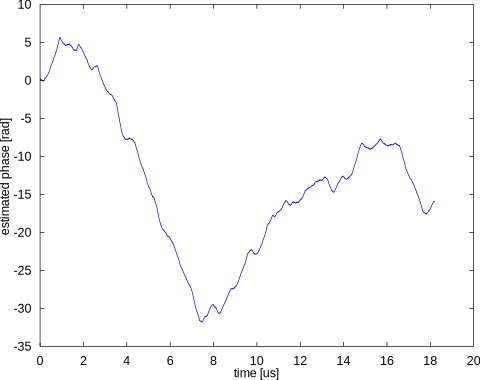
\includegraphics[width=0.8\textwidth]{figures/matlab/res_450_qam4_phase_est}
      \begin{block}{Time Comparison}
        \begin{description}
        \item[@1.8 GS/s] 1800 symbols per 1 $\mu \text{s}$
        \item[CIFS] 2 $\mu \text{s}$
        \end{description}
      \end{block}
    \end{column}
  \end{columns}
\end{frame}

\begin{frame}{Frame Structure}
  \begin{figure}
    \centering
    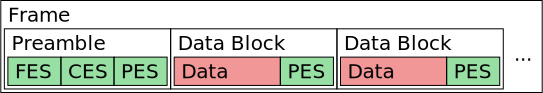
\includegraphics[width=0.7\textwidth]{figures/frame_struct}
  \end{figure}

  \begin{figure}
    \centering
    \begin{tabular}{|c|c|c|}
      \hline
      Modulation of Data Fiels & QAM-4 & QAM-256 \\ \hline
      Modulation of Estimation Fields & \mc{2}{BPSK} \\ \hline
      Length of FES field & \mc{2}{256 symbols} \\ \hline
      Length of CES field & \mc{2}{1152 symbols} \\ \hline
      Length of PES field & \mc{2}{32 symbols} \\ \hline
      Length of Data Block & \mc{2}{147 symbols} \\ \hline
      Length of Data Field & \mc{2}{115 symbols} \\ \hline
      Length of Data Field & 230 bits & 920 bits \\ \hline
    \end{tabular}
  \end{figure}
\end{frame}

\begin{frame}{Result at Symbol Rate of 450 MS / s}
  \begin{columns}[T]
    \begin{column}{.4\textwidth}
      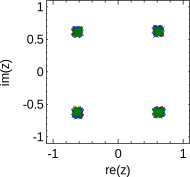
\includegraphics[width=\textwidth]{figures/matlab/res_450_qam4_cp_corr_pcorr_initial} \\
      \includegraphics[width=\textwidth]{figures/matlab/res_450_qam256_cp_corr_pcorr_initial}
    \end{column}
    \begin{column}{.6\textwidth}
      \begin{block}{Error Vector Magnitude}
        \begin{tabular}{|l|r@{}l|r@{}l|r@{}l|}
          \hline
          & \mc{2}{$\text{EVM}_\text{D}$} \\ \hline
          channel correction &   1&.52 \\ \hline
          + phase noise      & -23&.88 \\ \hline
          + initial phase    & {\bf-30}&.29 \\ \hline
        \end{tabular}
      \end{block}
      \begin{block}{Raw Data Speed}
        QAM-4: $0.838 \;\frac{\text{GiBit}}{\text{s}}$ \\
        QAM-256: $3.353 \;\frac{\text{GiBit}}{\text{s}}$
      \end{block}
    \end{column}
  \end{columns}
\end{frame}



\begin{frame}{Summary}
\end{frame}

\begin{frame}{Conclusion}
  \begin{itemize}
  \item Multi-Gigabit Throughput is possible
  \item Sub-Nyquist Sampling works well
  \item Phase Noise correction is essential
  \end{itemize}
\end{frame}

\begin{frame}{Outlook}
  \begin{itemize}
  \item Framework can be used for further simulations
  \item FPGA is ready to be extended
  \end{itemize}
\end{frame}

\end{document}
